\chapter{Phương pháp đề xuất}

\section{Tổng quan hệ thống}

Với mục đích tự động hóa quy trình nhận dạng ký tự quan học (OCR) và sinh câu hỏi trắc ngiệm (MCQ), nghiên cứu này đề xuất và phát triển hệ thống phần mềm Openlet. Nhờ việc các tài liệu học tập được số hóa thông quá các bài tập trắc nghiệm tạo sinh, đội ngũ giáo viên được giảm bớt gánh nặng công việc và người học có thể thuận tiện cho việc ôn tập. Khảo sát nghiên cứu hiện hành cho thấy một sự đánh đổi lớn về mặt công nghệ: việc triển khai các sLLM mã nguồn mở giúp tối ưu hóa chi phí vận hành nhưng lại dẫn tới một đánh đổi lớn về mặt chất lượng của câu hỏi được sinh ra, các câu hỏi không đủ độ khó và các đáp án nhiễu không có tính sư phạm. Ngược lại, các LLM thương mại mã nguồn đóng dù đảm bảo chất lượng đầu ra vượt trội hoàn toàn nhưng lại có chi phí quá cao để có thể ứng dụng đại trà trong môi trường giáo dục. Nhằm giải quyết bài toán trên, hệ thống Openlet được nghiên cứu và phát triển với kiến trúc đa tác tử, là tập hợp gồm các sLLM phối hợp hoạt động. Bằng cách chia nhỏ quy trình suy luận phức tạp thành chuỗi các tác vụ vi mô cho từng sLLM riêng việt, hệ thống vừa tận dụng được lợi thế chi phí thấp của các mô hình nhỏ mà vừa cải thiện được chất lượng các mô hình.

Về mặt tổng quan, ứng dụng Openlet được chia thành 4 mô-đun chính:

\begin{enumerate}
    \item \textbf{Mô-đun sinh câu hỏi (Question Generation Module):} Đây là thành phần cốt lõi của nghiên cứu. Mô-đun này sẽ tiếp nhận dữ liệu đầu vào là một đoạn văn bản tiếng Anh thuần túy và có đầu ra mong muốn là các câu hỏi trắc nghiệm gồm cả 3 loại trong thang đo Bloom sửa đổi về đoạn văn bản. Nghiên cứu này sẽ thực nghiệm và so sánh hai phương pháp sinh câu hỏi từ sLLM điển hình nhất là phương pháp truy vấn đơn và phương pháp đa tác tử. Việc tích hợp đồng thời hai cơ chế này hướng tới mục đích thiết lập một hệ thống đánh giá về chất lượng và chi phí trong điều kiện vận hành thực tế.

    \item \textbf{Mô-đun Tiền xử lý Hình ảnh và Nhận dạng Ký tự (OCR \& Image Processing Module):} Thực tế cho thấy nguồn dữ liệu đầu vào của giáo viên và học sinh thường tồn tại dưới dạng các hình ảnh chụp từ một tài liệu học tập như sách giáo khoa, đề thi. Mô-đun này có nhiệm vụ trích xuất nội dung dưới dạng văn bản từ nguồn dữ liệu này để phục vụ cho Mô-đun sinh câu hỏi. Với mục đích đánh giá độ chính xác của các VLM hiện hành trong môi trường thực tế, nghiên cứu đã triển khai một quy trình tăng cường dữ liệu nhiễu (Data Augmentation). Quy trình này cho phép mô phỏng sự suy giảm tín hiệu thị giác như: cường độ ánh sáng kém, vết ố vàng, nhòe mực hoặc các biến dạng vật lý của bề mặt giấy. Từ đó giúp nghiên cứu có thể đánh giá được khả năng của từng VLM.

    \item \textbf{Mô-đun Đánh giá Chất lượng Câu hỏi Tự động (Evaluation Module):} Yêu cầu bắt buộc đối với các hệ thống sinh câu hỏi tự động là cần có các tiêu chuẩn kiểm định chất lượng đầu ra. Để có thể kiểm tra và đánh giá dữ liệu đầu ra một cách hoàn toàn tự động, nghiên cứu này sử dụng kỹ thuật đánh giá dựa trên LLM (LLM-as-a-judge). Nghiên cứu sử dụng bộ khung đánh giá gồm bốn tiêu chí sư phạm: Khả năng giải quyết được dựa trên ngữ cảnh (Solvability); Chất lượng của phương án nhiễu (Distractor Quality); Sự đáp ứng thang đo nhận thức (Alignment) và Sự rõ ràng của câu hỏi (Clarity).

    \item \textbf{Mô-đun Ứng dụng Web tương tác (Web Application Module):} Nhằm hiện thực hóa các kết quả nghiên cứu lý thuyết từ môi trường học thuật sang ứng dụng, nghiên cứu đã phát triển một ứng dụng Web giáo dục hiện đại - Openlet. Ứng dụng này cho phép giáo viên đăng tải các ảnh chụp tài liệu, sau đó hệ thống sẽ tự động trích xuất văn bản từ ảnh rồi tác các câu hỏi trắc nghiệm dưới một bài kiểm tra trực tuyến. Nhờ đó, học sinh có thể tham gia làm bài trực tiếp trên nền tảng một cách thuận tiện.

\end{enumerate}

Nhờ việc nghiên cứu và phát triển các mô-đun trên, hệ thống Openlet đã có thể trở thành một giải pháp công nghệ giáo dục (Ed-Tech) có giá trị thực tiễn cao. Bắt đầu từ một hình ảnh chụp tài liệu, được trích xuất văn bản, sinh câu hỏi trắc nghiệm và cuối cùng trở thành một học liệu số hóa đáp ứng các quy chuẩn sư phạm chuyên sâu.

\section{Phương pháp sinh câu hỏi trắc nghiệm}
Trong nghiên cứu này, để có thể hướng dẫn các sLLM và LLM thực hiện các yêu cầu sinh câu hỏi trắc nghiệm, nghiên cứu đã triển khai và so sánh hai phương pháp: Phương pháp chỉ dẫn đơn và phương pháp đa tác tử.

\subsection{Phương pháp chỉ dẫn đơn}
Phương pháp chỉ dẫn đơn thực hiện cấu trúc hóa toàn bộ các ràng buộc về nghiệp vụ, quy định về định dạng đầu ra trong một chỉ dẫn duy nhất. Chỉ dẫn này bao gồm các thông tin về vai trò của LLM, các định nghĩa chi tiết của ba cấp độ tư duy, các tiêu chuẩn để tạo ra đáp án nhiễu, và các quy định về định dạng đầu ra. Cụ thể, dữ liệu đầu ra bắt buộc phải xuất dưới dạng văn bản Markdown hoặc JSON cố định bao gồm các trường như: mã định danh (ID), nội dung câu hỏi (Question), bốn phương án độc lập (A, B, C, D) và đáp án chính xác (Answer). Toàn bộ quy trình này diễn ra trong một lần gọi duy nhất và hệ thống nhận được kết quả là danh sách các câu hỏi của cả ba cấp độ tư duy.

\textbf{Đánh giá tính khả dĩ của phương pháp:}

Lợi thế cốt lõi của phương pháp này là tối ưu hóa chi phí tính toán bằng giới hạn giao tiếp với bên cung cấp dịch vụ LLM bằng một lệnh gọi API duy nhất giúp giảm triệt độ số lượng token cần xử lý và duy trì độ trễ ở mức cực thấp.

Tuy nhiên, việc nén hàng loạt các quy tắc nghiệp vụ và định nghĩa của ba cấp độ vào một không gian suy luận đơn lẻ gây ra hiện tượng pha loãng ngữ cảnh (context dilution). Kết quả thực nghiệm cho thấy LLM thường thất bại trong việc phân biệt giữa các độ khó và cấp độ nhận thức, từ đó dẫn đến việc LLM có xu hướng sinh ra các câu hỏi Cấp độ 1 thay vì Cấp độ 3 như yêu cầu. Không những thế, do thiếu đi sự giám sát, các câu hỏi sinh ra có thể vi phạm những quy định sư phạm như chứa nhiều hơn một đáp án đúng, câu hỏi mơ hồ hay đáp án nhiễu quá  lộ liễu.

\subsection{Phương pháp đa tác tử}
Nhằm giải quyết giới hạn không gian ngữ cảnh của phương pháp truy vấn đơn, hệ thống tích hợp kiến trúc điều khiển luồng dựa trên đồ thị. Quy trình sinh câu hỏi được chia nhỏ thành các nút chức năng. Mỗi nút sẽ vận hành một phiên bản sLLM có cấu hình chuyên biệt cho một tác vụ. Các tác tử này giao tiếp với nhau thông qua một cấu trúc dữ liệu trạng thái chung. Khối dữ liệu này vận chuyển văn bản nguồn, kết quả phân tích trung gian và các mảng dữ liệu tạm thời giữa các luồng.

% \begin{figure}
%     \centering
%     \includesvg[width=1\linewidth]{figures/workflow.svg}
%     \caption{Kiến trúc hệ thống đa tác tử sinh câu hỏi trắc nghiệm từ văn bản}
%     \label{fig:placeholder}
% \end{figure}

Quy trình hoạt động của hệ thống đa tác tử gồm khối chức năng sau:

\begin{enumerate}

    \item \textbf{Khối tác tử Phân tích toàn cảnh (Analyzer Agent):} Đây là thành phần xử lý đầu tiên, có nhiệm vụ là trích xuất những dữ liệu quan trọng từ đoạn văn bản: các sự kiện chính, thực thể trọng tâm, luận điểm của tác giả và các thông điệp khái quát. Đầu ra sẽ được lưu vào biến trạng thái dùng chung và được truyền xuống các nốt tiếp theo. Tác dung chính của nốt này thực hiện một bước suy luận, phân tích dữ liệu tương tự mô hình Chain-of-Thought (CoT) nhằm tăng chất lượng kết quả đầu ra.

    \item \textbf{Khối các tác tử sinh câu hỏi (Generator Agents):} Luồng dữ liệu được chia tách song song vào ba tác tử đại diện cho ba mức nhận thức. Tác tử Cấp 1 có nhiệm vụ sinh các câu hỏi đọc hiểu đơn giản. Tác tử Cấp 2 lại chuyên biệt cho các câu hỏi về suy luận và tổng hợp. Trong khi Tác tử Cấp 3 có nhiệm vụ tạo ra các câu hỏi mang tính chất phản biển, mức độ logic cao hơn. Việc thu hẹp không gian nhiệm vụ giúp loại bỏ hoàn toàn hiện tượng chồng lấn, quá tải các quy tắc nghiệp vụ, đảm bảo độ chính xác trong việc xác định mức độ khó/dễ.

    \item \textbf{Khối tác tử Thẩm định (Validator Agent):} Khối này có vai trò kiểm định chất lượng của các câu hỏi do Tác tử trên tạo ra. Quá trình thẩm định được tham chiếu trên bốn tiêu chuẩn cốt lõi: Khả năng giải quyết dựa trên dữ kiện bài đọc (Solvability), Chất lượng phương án nhiễu (Distractor Quality), Sự bám sát cấp độ nhận thức (Alignment) và Sự rõ ràng của câu hỏi (Clarity). Bất kỳ thành phần nào của câu hỏi vi phạm quy chuẩn trên đều bị gắn định danh thất bại (FAIL), ví dụ như: câu hỏi lạc đề, nhiều hơn một đáp án đúng, đáp án sai quá rõ ràng. Đi kèm với nhãn thất bại này là một đoạn văn bản chưa dữ liệu phản hồi chi tiết, có nhiệm vụ nêu rõ nguyên nhân vi phạm nhằm giúp Tác tử tiếp theo sửa lỗi chính xác hơn.

    \item \textbf{Khối tác tử Hiệu chỉnh (Fixer Agent):} Các câu hỏi chưa nhãn thất bại sẽ lập tức được chuyển giao cho Tác tử Hiệu chỉnh nhằm thiết kế lại nội dung sao cho phù hợp. Thành phần cốt lõi quyết định chất lượng của đầu ra của tác tử này là biến lưu trữ lịch sử phản hồi. Khi một câu hỏi liên tục bị gán nhãn thất bại từ Tác tử Thẩm định, toàn bộ các phản hồi từ các vòng đánh giá trước sẽ được nhúng trực tiếp vào chỉ dẫn của Tác tử Hiệu chỉnh. Mảng dữ liệu lịch sử này giúp triệt tiêu nguy cơ mô hình ngôn ngữ rơi vào vòng lặp vì nó lặp lại các lỗi từ vòng trước.

    \item \textbf{Khối Hợp nhất (Merge Node):} Khối này có nhiệm vụ tổng hợp các câu hỏi được chấp nhận từ ba khối Thẩm định, đánh lại chỉ số và hợp nhất thành bộ câu hỏi hoàn chỉnh cuối cùng.
    
\end{enumerate}

\textbf{Đánh giá tính khả dĩ của phương pháp:}

Kiến trúc đa tác tử giúp tận dụng tối đa khả năng suy luận của các sLLM. Chất lượng câu hỏi sinh ra đạt độ chính xác cao về mặt phân loại nhận thức . Vòng lặp thẩm định và hiệu chỉnh giúp loại bỏ các lỗi sư phạm và logic. Hạn chế của kiến trúc này là tiêu thụ lượng token lớn và có độ trễ cao hơn phương pháp chỉ dẫn đơn.

\section{Quy trình OCR}
Trong môi trường giáo dục thực tế, dữ liệu học tập rất hiếm khi tồn tại dưới các định dạng số hóa thuần túy như văn bản mà thường dưới dạng ảnh chụp sách giáo khoa, tài liệu in, đề thi, hoặc ghi chép tay. Nhằm đáp ứng nhu cầu trích xuất thông tin từ các dạng văn bản này, đồng thời triển khai một quy trình thử nghiệm có kiểm soát và đánh giá các VLM, nghiên cứu đã xây dựng một quy trình OCR khép kín. 

Thay vì thu thập dữ liệu ảnh chụp văn bản thủ công - phương pháp vốn tồn tại nhược điểm về chi phí gán nhãn và thiếu sự kiểm soát đối với mức độ nhiễu - hệ thống triển khai một quy trình sinh dữ liệu tổng hợp. Quá trình này là đảo ngược thứ tự của bài toàn OCR truyền thống trong giai đoạn chuẩn bị dữ liệu: hệ thống bắt đầu với một đoạn văn bản chuẩn lấy từ bộ dữ liệu nghiên cứu, sau đó chủ động tạo ra các hình ảnh chứa các đoạn văn bản đó và cuối cùng là thêm các tác nhân gây nhiễu trong môi trường thực tế vào ảnh vừa tạo. Nhờ đóm nghiên cứu có thể thực hiện đánh giá độ chính xác và hiệu năng các VLM trong ngữ cảnh thực tế mà không cần tốn tài nguyên thu thập dữ liệu và gán nhãn.

\begin{figure}
    \centering
    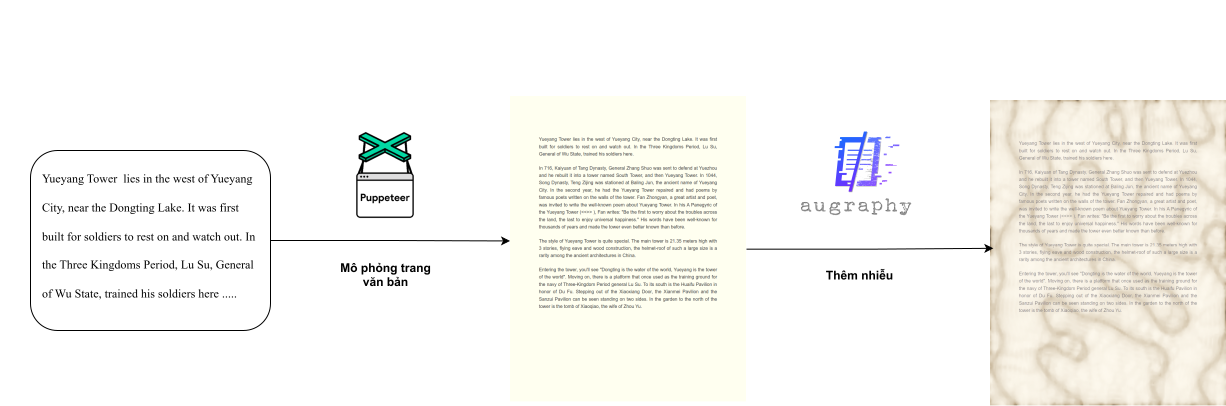
\includegraphics[width=1\linewidth]{figures/augmentation-pipeline.png}
    \caption{Sơ đồ quy trình tăng cường dữ liệu ảnh nhiễu}
    \label{fig:placeholder}
\end{figure}

\subsection{Sinh ảnh sạch từ văn bản}

Tác vụ đầu tiên trong quy trình là tạo ra các hình ảnh kỹ thuật số mang độ sắc nét tuyệt đối từ các đoạn văn bản đầu vào. Để đảm bảo tính đa dạng về mặt thị giác và kiểm thử, nghiên cứu không sử dụng các thư viện vẽ chữ trên ảnh như PIL mà tích hợp công cụ trình duyệt không giao diện (headless browser) thông qua thư viện Pyppeteer. Nhờ đó, nghiên cứu có thể tận dụng sức mạnh và độ thuận tiện của CSS và DOM để kiểm soát chính xác cấu trúc của hình ảnh được tạo ra.

Quá trình tạo ảnh sạch được thực hiện thông qua ba bước sau:

\begin{enumerate}
    \item \textbf{Cài đặt các tham số định dạng không gian và kiểu chữ:} Hệ thống tự động lựa chọn ngẫu nhiên các khung kích thước tiêu chuẩn trong thực tế như giấy in (A4, A5, US Letter), tỷ lệ màn hình điện tử (FHD, HD), hoặc định dạng truyền thông xã hội (Facebook Status, Twitter Post). Phông chữ được lựa chọn ngẫu nhiên từ một danh sách cài đặt sẵn thu thập trực tiếp từ Google Fonts. Danh sách này được phân loại thành hai nhóm chính bao gồm nhóm phông chữ in chuẩn (Roboto, Merriweather) để mô phỏng sách giáo khoa, tài liệu in ấn, và nhóm phông chữ viết tay (như Dancing Script, Caveat, Mali) nhằm tái tạo gần đúng chữ viết tay từ các bản ghi chép của giáo viên hoặc học sinh. Ngoài ra, các tham số hiển thị khác nhau độ đậm, màu chữ và màu nền cũng được khởi tạo ngẫu nhiên để đảm bảo tính đa dạng.

    \item \textbf{Thuật toán tính toán mật độ hiển thị:} Sau khi có các tham số hiển thị cần thiết, hệ thống sẽ đánh giá mật độ chữ trên diện tích của ảnh. Dựa trên tỷ lệ này, thuật toán sẽ quy định số lượng cột văn bản một cách linh hoạt (từ 1 đến 3 cột), khoảng cách lề (padding), độ giãn dòng (line height) và khoảng cách giữa các đoạn (paragraph spacing). Cơ chế này giúp đánh giả khả năng nhận diện các đoạn văn có cấu trúc phức tạp, nhiều cột của các mô hình.

    \item \textbf{Thuật toán tự động khớp khung hình:} Thành phần này giúp giải quyết vấn đề lỗi tràn viền hoặc cắt xén chữ khi hệ thống chỉ chụp ảnh màn hình của trang đầu tiên cho kết quả đầu ra. Quá trình tự động khớp diễn ra sau khi tài liệu HTML/CSS được khởi tạo, khi đó thuật toán được nhúng trong một thẻ Javascript sẽ tự động điều chỉnh cơ chữ sao cho toàn bộ nội dung trang sẽ nằm gọn trong màn hình (không kích hoạt hiển thị thanh cuộn). Cuối cùng, Pyppeteer sẽ tiến hành chụp lại toàn bộ khung hình và lưu trữ dưới dạng tệp hình ảnh.
    
\end{enumerate}

Việc tự động hóa toàn bộ quy trình cho phép hệ thống Openlet tạo ra hàng loạt hình ảnh mang dữ liệu chính xác tuyệt đối ở tốc độ vào, làm dữ liệu đầu vào cho bước xử lý nhiễu tiếp theo.

\subsection{Tạo dữ liệu ảnh nhiễu trong thực tế}

Trong thực tế, ảnh chụp tài liệu từ thiết bị di động của người dùng rất hiếm khi đạt được chất lượng quang học lý tưởng. Sự tụt giảm chất lượng này có thể đến từ nhiều tác động ngẫu nhiên từ môi trường như: điều kiện chiếu sáng kém, chất lượng giấy không tốt, độ phân giải của camera thấp, hoặc các tác động cơ học như nếp gấp và vết mực nhòe. Để có thể mô phỏng gần đúng các điều kiện nhiễu trong thực tế, hệ thống tiến hành  giả lập nhiễu (Data Augmentation) dựa trên lượng ảnh sạch đã tạo ra từ bước trên.

Nghiên cứu sử dụng thư viện Augraphy được thiết kế đặc thù cho các bài toán mô phỏng nhiễu của các tài liệu vật lý. Hệ thống thiết lập một tổ hợp các cơ chế gây nhiễu sau:

\begin{itemize}
    \item Về mặt chất liệu in ấn, hệ thống mô phỏng các lỗi cơ học của thiết bị in ấn bằng cách thêm vào hình ảnh các dải nhiễu cấu trúc như nhòe mực, chữ nét đứt hoặc mất chữ do tình trạng cạn mực. Nền ảnh gốc cũng được chỉnh sửa thành các bề mặt chất liệu khác nhau như thêm các họa tiết, vết ố vàng hoặc chèn các dòng chữ chìm. Các cơ chế này sẽ yêu cầu VLM phải sở hữu khả năng phân tách giữa các tín hiệu thông tin và lớp vật liệu nhiễu một cách chính xác.

    \item Về mặt quang học và các yếu tố con người, hệ thống sử dụng các biến đổi như thay đổi sự phân bố của ánh sáng, bóng đổ vật lý, nhiễu hạt do chụp trong điều kiện thiếu sáng, và hiện tượng lóa sáng. Hệ thống tích hợp thêm các lỗi kỹ thuật như lỗi nén ảnh quản học, sự sai lệch kênh màu, viền đen do từ máy photocopy, cùng các biến dạng hình học như giấy bị nhăn nhúm hoặc văn bản bị che khuất bởi gáy sách. Không chỉ thế, hệ thống còn mô phỏng các tác động thủ công từ người học như nét gạch chân, tô bằng bút dạ quang hoặc các nét vẽ nguệch ngoạc, ngẫu nhiên đề trực tiếp lên văn bản gốc.

    
    
\end{itemize}

Mỗi văn bản đầu vào đều được chỉnh sửa thành một phiên bản định dạng vật lý hoàn toàn khác biệt. Nhờ đó, nghiên cứu có thể đánh giá chính xác sức mạnh và hiệu suất của từng mô hình OCR trong môi trường thực tế.

\begin{figure}
    \centering
    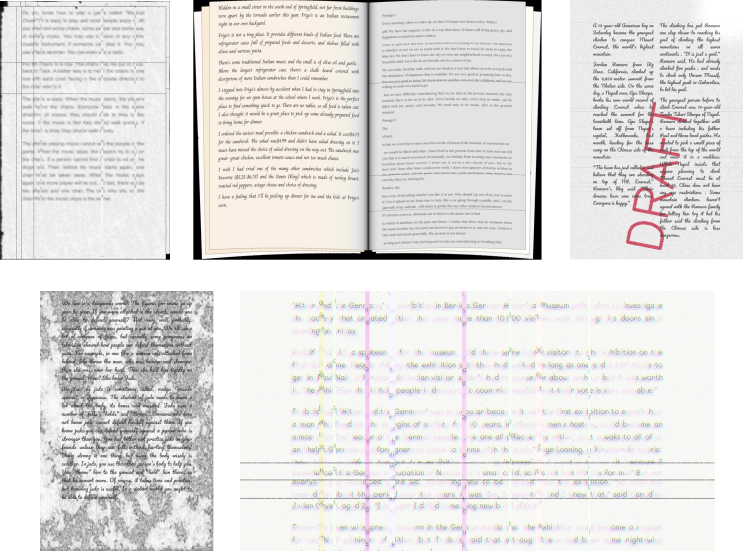
\includegraphics[width=1\linewidth]{figures/augmentation-samples.png}
    \caption{Các mẫu ảnh tài liệu tổng hợp sau khi thêm nhiễu}
    \label{}
\end{figure}

\subsection{Nhận dạng văn bản từ ảnh}

Giai đoạn cuối của quy trình tập trung vào việc trích xuất văn bản từ các tập dữ liệu ảnh (bao gồm cả ảnh sạch và ảnh nhiễu) thông qua API. Thay vì tự triển khai các mô hình OCR đòi hỏi tài nguyên phần cứng máy tính khổng lồ, hệ thống sử dụng các nền tảng trung gian như OpenRouter và Novita AI. Các hệ thống này cho phép thay đổi linh hoạt các mô hình và tiếp cận tới các OCR tiên tiến như PaddleOCR hay DeepSeek OCR.

\section{Phương pháp đánh giá chất lượng câu hỏi}

Bất kỳ một hệ thống sinh tự động nào cũng yêu cầu một cơ chế đánh giá độ tin cậy và mức độ hiệu quả của dữ liệu đầu ra. Đối với bài toán sinh câu hỏi trắc nghiệm tự động (AMCQG), các thang đo truyền thống như BLEU hay ROUGE tỏ ra hoàn toàn kém hiệu quả và không đáng tin cậy, lý do chính là chúng chỉ so sánh và đối chiếu sự trùng lặp từ vựng bề mặt mà bỏ quá tính sư phạm và ý nghĩa thực tế của câu hỏi. Để giải quyết vấn đề này, nghiên cứu phát triển một khung đánh giá tự động dựa trên các tiêu chí sư phạm kết hợp với phương pháp dùng LLM để đánh giá kết quả đầu ra (LLM-as-a-Judge).

\subsection{Các tiêu chí đánh giá}

Để có thể thẩm định được chất lượng của một câu hỏi trắc nghiệm, hệ thống sử dụng bốn tiêu chí độc lập. Mỗi tiêu chí đo lường một khía cạnh sư phạm của câu hỏi, đảm bảo đầu ra thỏa mãn các yêu cầu khắt khe của giáo dục:

\begin{enumerate}
    \item \textbf{Khả năng giải quyết dựa trên ngữ cảnh (Solvability):} Tiêu chí này kiểm định tính đóng của không gian thông tin. Theo lý thuyết, một câu hỏi đạt chuẩn Solvability bắt buộc phải chứa duy nhất một đáp án đúng, và đáp án này phải được suy luận hoàn toàn ra từ các thông tin nằm bên trong đoạn văn bản được cung cấp. Không chỉ vậy, yêu cầu này còn nghiêm cấm hiện tượng ảo giác của LLM khi sinh ra các câu hỏi mà câu trả lời tạo ra từ kiến thức bên ngoài. Điều này dẫn đến việc nếu người đọc không thể trả lời câu hỏi ngay trên văn bản đầu vào, câu hỏi đó hoàn toàn vi phạm nguyên tắc này.

    \item \textbf{Chất lượng phương án nhiễu (Distractor Quality):} Tiêu chí này đóng vai trò kiểm định độ sắc bén của một câu hỏi. Một phương án sai hợp lệ phải đồng thời thỏa mãn hai điều kiện: Trái ngược hoàn toàn so với đáp án đúng về mặt bản chất, không tạo ra tránh cãi hoặc tính đa nghĩa; Có khả năng đánh lừa đối với những người học không nắm vững kiến thức. Các lựa chọn nhiễu hiển nhiên sai, lệch ngữ cảnh thường sẽ bị loại bỏ.

    \item \textbf{Độ bám sát phân loại nhận thức (Alignment):} Tiêu chí này đo lường mức độ nhận thức hay độ khó của câu hỏi sinh ra có đúng với cấu hình yêu cầu từ trước hay không. Hệ thống sẽ thực hiện đối chiếu và đánh giá các câu hỏi được sinh ra với thang đo Bloom. Nếu LLM được giao nhiệm vụ sinh ra một câu hỏi Cấp 3 mà lại đưa ra một câu hỏi Cấp 1 thì đó là vi phạm tính Alignment do sự lệch pha về độ sâu nhận thức.

    \item \textbf{Độ tường minh ngữ nghĩa (Clarity):} Đây là tiêu chí đánh giá mức độ tường minh của nội dung câu hỏi và các đáp án. Sự tường minh đảm bảo người học không bị cản trở bởi cấu trúc câu hỏi lủng củng hay sử dụng các từ ngữ mơ hồ không rõ ràng từ LLM.
    
\end{enumerate}

\subsection{Phương pháp LLM-as-a-Judge}

Để có thể khắc phục các hạn chế cố hữu của các thang đo truyền thống, nghiên cứu này áp dụng phương pháp sử dụng LLM để đánh giá kết quả đầu ra (LLM-as-a-Judge). Cụ thể, phương pháp này thiết kế một LLM chuyên biệt cho vai trò làm giám khảo. Đầu vào của LLM này gồm ba dữ liệu: văn bản nguồn, bộ câu hỏi cần kiểm định, và bộ tiêu chuẩn đánh giá chi tiết theo từng cấp độ nhận thức. Đầu ra sẽ là điểm số cụ thể cho từng tiêu chí.

Về mặt kỹ thuật thiết kế chỉ dẫn, quy trình đánh giá bắt buộc phải tích hợp kỹ thuật Chain-of-Thought. Nhằm đảm bảo tính chính xác và minh bạch của kết quả thẩm định, hệ thống bắt buộc LLM giám khảo phải đưa ra một chuỗi lập luận logic để giải thích cho quá trình đánh giá trước khi đưa ra điểm số cuối cùng cho mỗi tiêu chí. Cấu trúc đánh giá cho từng tiêu chí bao gồm:

\begin{enumerate}
    \item \textbf{Khả năng giải quyết (Solvability):} LLM giám khảo sẽ kiểm tra xem câu hỏi có thể được trả lời nếu chỉ dựa vào văn bản được cung cấp hay không. Tiếp theo, mô hình sẽ kiểm tra tính duy nhất của đáp án đúng, đồng thời đánh giá tính sai lệch của ba đáp án còn lại. Kết quả trả về là 1 nếu câu hỏi đáp ứng tiêu chí và 0 nếu ngược lại.

    \item \textbf{Chất lượng phương án nhiễu (Distractor Quality):} Mô hình giám khảo sẽ thực hiện phân tích kỹ thuật tạo đáp án nhiễu. Mỗi cấp độ sẽ có các tiêu chí riêng để đánh giá: mệnh đề đúng một phần hoặc các thông tin thực tế nhưng không liên quan đến chuỗi suy luận. Điểm số của tiêu chí này là từ 1 đến 5 điểm.

    \item \textbf{Độ bám sát (Alignment):} Mô hình sẽ thực hiện đối chiếu câu hỏi đầu vào với các định nghĩa và tiêu chuẩn của cấp độ được yêu cầu. Nếu câu hỏi sinh ra có mức độ nhận thức và độ khó như yêu cầu, LLM sẽ gán điểm số là 1 và 0 nếu không đạt yêu cầu.

    \item \textbf{Độ tường minh (Clarity):} Với tiêu chí này, mô hình giám khảo sẽ rà soát cấu trúc ngữ pháp và tính đơn nghĩa của câu hỏi cùng các phương án lựa chọn. Các vấn đề liên quan đến chính tả, lặp từ hay cách diễn đạt mơ hồ, dễ gây hiểu lầm sẽ được gán điểm 0.
    
\end{enumerate}

\begin{figure}
    \centering
    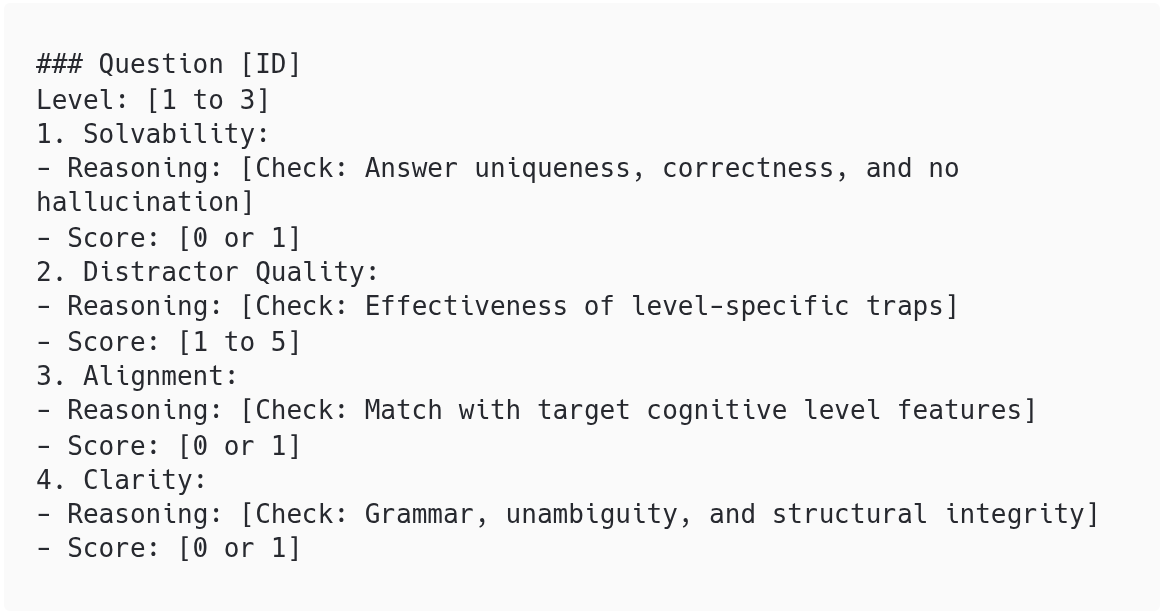
\includegraphics[width=1\linewidth]{figures/llm-as-a-judge.png}
    \caption{Định dạng đầu ra tích hợp Chain-of-Thought}
    \label{fig:placeholder}
\end{figure}

\section{Ứng dụng minh họa - Openlet}
\subsection{Kiến trúc hệ thống}
\subsection{Luồng hoạt động}